\documentclass[12pt]{article}
\usepackage[letterpaper, left=13mm, right=13mm, top=20mm, bottom=20mm,
  headheight=15pt, headsep=5mm, footskip=10mm]{geometry}
\usepackage[T1]{fontenc}
\usepackage[utf8]{inputenc}
\usepackage{tgheros}
\renewcommand{\familydefault}{\sfdefault}
\usepackage{fancyhdr}
\usepackage{tikz}
\usetikzlibrary{arrows.meta}
\pagestyle{fancy}
\fancyhf{}
\lhead{\small Week NN / Poisoned cookie / Grades 2--3}
\lfoot{\small Bellingham Math Circle / Week NN / NN-23-v1}
\rfoot{\small \thepage}
\renewcommand{\headrulewidth}{0.4pt}
\renewcommand{\footrulewidth}{0pt}
\setlength{\parindent}{0pt}
\setlength{\parskip}{0pt}
\newcommand{\prob}[1]{\par\textbf{Problem #1:}~}
\raggedright
\begin{document}
Two players take turns. On your turn, put the corner of the bite card on any cookie and eat every cookie under the card. That is the chosen cookie and every cookie above it or to its right, including those up and to the right. Whoever has to eat the poison cookie in the bottom-left corner loses. To record a bite, draw an X on the chosen cookie.\par\vspace{4mm}
{\centering 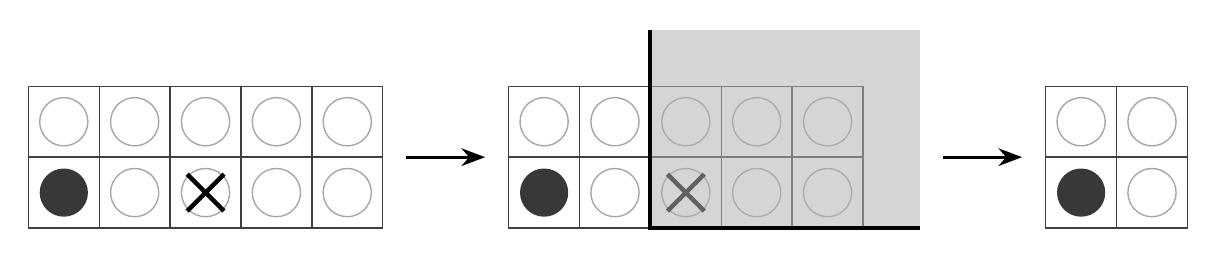
\begin{tikzpicture}[x=1mm, y=1mm]
\draw[line width=0.5pt, black!75] (0,0) rectangle ++(9,9);
\fill[black!78] (4.5,4.5) circle (3.06);
\draw[line width=0.5pt, black!75] (9,0) rectangle ++(9,9);
\draw[line width=0.5pt, black!35] (13.5,4.5) circle (3.06);
\draw[line width=0.5pt, black!75] (18,0) rectangle ++(9,9);
\draw[line width=0.5pt, black!35] (22.5,4.5) circle (3.06);
\draw[line width=0.5pt, black!75] (27,0) rectangle ++(9,9);
\draw[line width=0.5pt, black!35] (31.5,4.5) circle (3.06);
\draw[line width=0.5pt, black!75] (36,0) rectangle ++(9,9);
\draw[line width=0.5pt, black!35] (40.5,4.5) circle (3.06);
\draw[line width=0.5pt, black!75] (0,9) rectangle ++(9,9);
\draw[line width=0.5pt, black!35] (4.5,13.5) circle (3.06);
\draw[line width=0.5pt, black!75] (9,9) rectangle ++(9,9);
\draw[line width=0.5pt, black!35] (13.5,13.5) circle (3.06);
\draw[line width=0.5pt, black!75] (18,9) rectangle ++(9,9);
\draw[line width=0.5pt, black!35] (22.5,13.5) circle (3.06);
\draw[line width=0.5pt, black!75] (27,9) rectangle ++(9,9);
\draw[line width=0.5pt, black!35] (31.5,13.5) circle (3.06);
\draw[line width=0.5pt, black!75] (36,9) rectangle ++(9,9);
\draw[line width=0.5pt, black!35] (40.5,13.5) circle (3.06);
\draw[line width=1.6pt] (20.16,2.16) -- (24.84,6.84) (20.16,6.84) -- (24.84,2.16);
\draw[-{Stealth[length=3mm]}, line width=1pt] (48,9) -- ++(10,0);
\draw[line width=0.5pt, black!75] (61,0) rectangle ++(9,9);
\fill[black!78] (65.5,4.5) circle (3.06);
\draw[line width=0.5pt, black!75] (70,0) rectangle ++(9,9);
\draw[line width=0.5pt, black!35] (74.5,4.5) circle (3.06);
\draw[line width=0.5pt, black!75] (79,0) rectangle ++(9,9);
\draw[line width=0.5pt, black!35] (83.5,4.5) circle (3.06);
\draw[line width=0.5pt, black!75] (88,0) rectangle ++(9,9);
\draw[line width=0.5pt, black!35] (92.5,4.5) circle (3.06);
\draw[line width=0.5pt, black!75] (97,0) rectangle ++(9,9);
\draw[line width=0.5pt, black!35] (101.5,4.5) circle (3.06);
\draw[line width=0.5pt, black!75] (61,9) rectangle ++(9,9);
\draw[line width=0.5pt, black!35] (65.5,13.5) circle (3.06);
\draw[line width=0.5pt, black!75] (70,9) rectangle ++(9,9);
\draw[line width=0.5pt, black!35] (74.5,13.5) circle (3.06);
\draw[line width=0.5pt, black!75] (79,9) rectangle ++(9,9);
\draw[line width=0.5pt, black!35] (83.5,13.5) circle (3.06);
\draw[line width=0.5pt, black!75] (88,9) rectangle ++(9,9);
\draw[line width=0.5pt, black!35] (92.5,13.5) circle (3.06);
\draw[line width=0.5pt, black!75] (97,9) rectangle ++(9,9);
\draw[line width=0.5pt, black!35] (101.5,13.5) circle (3.06);
\draw[line width=1.6pt] (81.16,2.16) -- (85.84,6.84) (81.16,6.84) -- (85.84,2.16);
\fill[black!30, opacity=0.55] (79,0) rectangle (113.2,25.2);
\draw[line width=1.4pt] (113.2,0) -- (79,0) -- (79,25.2);
\draw[-{Stealth[length=3mm]}, line width=1pt] (116.2,9) -- ++(10,0);
\draw[line width=0.5pt, black!75] (129.2,0) rectangle ++(9,9);
\fill[black!78] (133.7,4.5) circle (3.06);
\draw[line width=0.5pt, black!75] (138.2,0) rectangle ++(9,9);
\draw[line width=0.5pt, black!35] (142.7,4.5) circle (3.06);
\draw[line width=0.5pt, black!75] (129.2,9) rectangle ++(9,9);
\draw[line width=0.5pt, black!35] (133.7,13.5) circle (3.06);
\draw[line width=0.5pt, black!75] (138.2,9) rectangle ++(9,9);
\draw[line width=0.5pt, black!35] (142.7,13.5) circle (3.06);
\end{tikzpicture}\par}\vspace{8mm}
\prob{1}It is your turn on each board. If you can make sure to win, however your partner plays, mark your first bite. If you can't, explain why.\par\vspace{5mm}
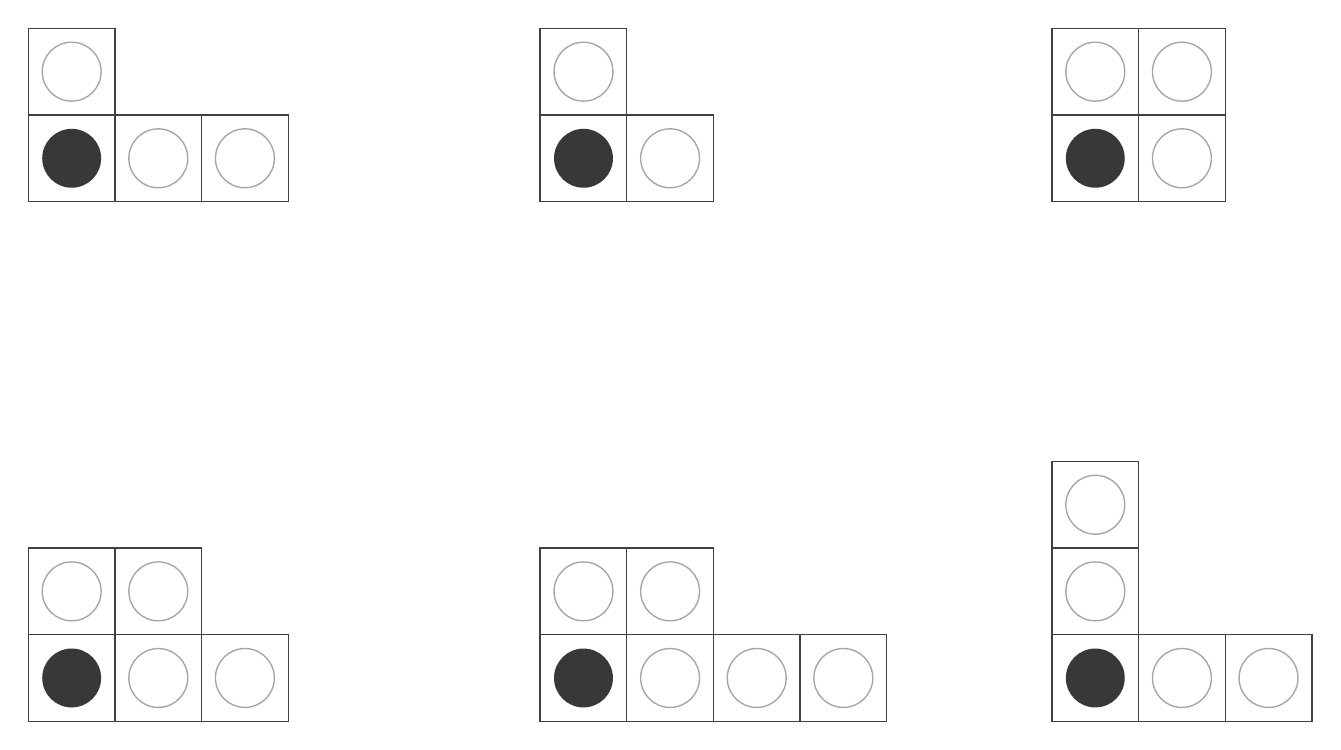
\begin{tikzpicture}[x=1mm, y=1mm]
\draw[line width=0.5pt, black!75] (0,-33) rectangle ++(11,11);
\fill[black!78] (5.5,-27.5) circle (3.74);
\draw[line width=0.5pt, black!75] (11,-33) rectangle ++(11,11);
\draw[line width=0.5pt, black!35] (16.5,-27.5) circle (3.74);
\draw[line width=0.5pt, black!75] (22,-33) rectangle ++(11,11);
\draw[line width=0.5pt, black!35] (27.5,-27.5) circle (3.74);
\draw[line width=0.5pt, black!75] (0,-22) rectangle ++(11,11);
\draw[line width=0.5pt, black!35] (5.5,-16.5) circle (3.74);
\draw[line width=0.5pt, black!75] (65,-33) rectangle ++(11,11);
\fill[black!78] (70.5,-27.5) circle (3.74);
\draw[line width=0.5pt, black!75] (76,-33) rectangle ++(11,11);
\draw[line width=0.5pt, black!35] (81.5,-27.5) circle (3.74);
\draw[line width=0.5pt, black!75] (65,-22) rectangle ++(11,11);
\draw[line width=0.5pt, black!35] (70.5,-16.5) circle (3.74);
\draw[line width=0.5pt, black!75] (130,-33) rectangle ++(11,11);
\fill[black!78] (135.5,-27.5) circle (3.74);
\draw[line width=0.5pt, black!75] (141,-33) rectangle ++(11,11);
\draw[line width=0.5pt, black!35] (146.5,-27.5) circle (3.74);
\draw[line width=0.5pt, black!75] (130,-22) rectangle ++(11,11);
\draw[line width=0.5pt, black!35] (135.5,-16.5) circle (3.74);
\draw[line width=0.5pt, black!75] (141,-22) rectangle ++(11,11);
\draw[line width=0.5pt, black!35] (146.5,-16.5) circle (3.74);
\draw[line width=0.5pt, black!75] (0,-99) rectangle ++(11,11);
\fill[black!78] (5.5,-93.5) circle (3.74);
\draw[line width=0.5pt, black!75] (11,-99) rectangle ++(11,11);
\draw[line width=0.5pt, black!35] (16.5,-93.5) circle (3.74);
\draw[line width=0.5pt, black!75] (22,-99) rectangle ++(11,11);
\draw[line width=0.5pt, black!35] (27.5,-93.5) circle (3.74);
\draw[line width=0.5pt, black!75] (0,-88) rectangle ++(11,11);
\draw[line width=0.5pt, black!35] (5.5,-82.5) circle (3.74);
\draw[line width=0.5pt, black!75] (11,-88) rectangle ++(11,11);
\draw[line width=0.5pt, black!35] (16.5,-82.5) circle (3.74);
\draw[line width=0.5pt, black!75] (65,-99) rectangle ++(11,11);
\fill[black!78] (70.5,-93.5) circle (3.74);
\draw[line width=0.5pt, black!75] (76,-99) rectangle ++(11,11);
\draw[line width=0.5pt, black!35] (81.5,-93.5) circle (3.74);
\draw[line width=0.5pt, black!75] (87,-99) rectangle ++(11,11);
\draw[line width=0.5pt, black!35] (92.5,-93.5) circle (3.74);
\draw[line width=0.5pt, black!75] (98,-99) rectangle ++(11,11);
\draw[line width=0.5pt, black!35] (103.5,-93.5) circle (3.74);
\draw[line width=0.5pt, black!75] (65,-88) rectangle ++(11,11);
\draw[line width=0.5pt, black!35] (70.5,-82.5) circle (3.74);
\draw[line width=0.5pt, black!75] (76,-88) rectangle ++(11,11);
\draw[line width=0.5pt, black!35] (81.5,-82.5) circle (3.74);
\draw[line width=0.5pt, black!75] (130,-99) rectangle ++(11,11);
\fill[black!78] (135.5,-93.5) circle (3.74);
\draw[line width=0.5pt, black!75] (141,-99) rectangle ++(11,11);
\draw[line width=0.5pt, black!35] (146.5,-93.5) circle (3.74);
\draw[line width=0.5pt, black!75] (152,-99) rectangle ++(11,11);
\draw[line width=0.5pt, black!35] (157.5,-93.5) circle (3.74);
\draw[line width=0.5pt, black!75] (130,-88) rectangle ++(11,11);
\draw[line width=0.5pt, black!35] (135.5,-82.5) circle (3.74);
\draw[line width=0.5pt, black!75] (130,-77) rectangle ++(11,11);
\draw[line width=0.5pt, black!35] (135.5,-71.5) circle (3.74);
\end{tikzpicture}\par\vspace{0mm}
\newpage
\prob{2}On each board, mark a first bite after which the first player can make sure to win.\par\vspace{5mm}
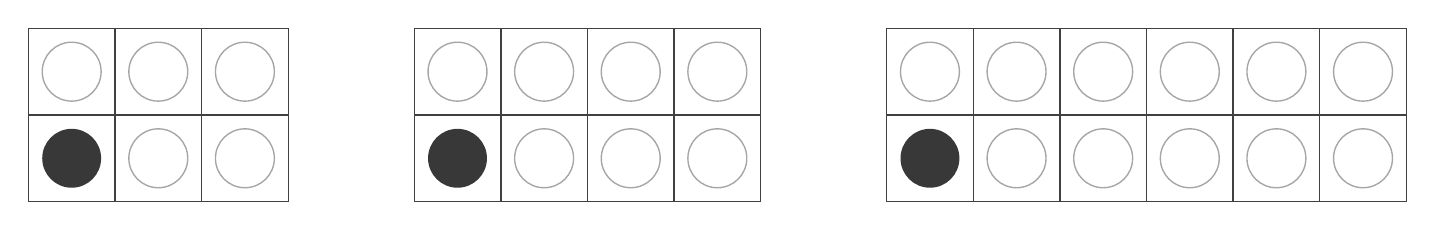
\begin{tikzpicture}[x=1mm, y=1mm]
\draw[line width=0.5pt, black!75] (0,0) rectangle ++(11,11);
\fill[black!78] (5.5,5.5) circle (3.74);
\draw[line width=0.5pt, black!75] (11,0) rectangle ++(11,11);
\draw[line width=0.5pt, black!35] (16.5,5.5) circle (3.74);
\draw[line width=0.5pt, black!75] (22,0) rectangle ++(11,11);
\draw[line width=0.5pt, black!35] (27.5,5.5) circle (3.74);
\draw[line width=0.5pt, black!75] (0,11) rectangle ++(11,11);
\draw[line width=0.5pt, black!35] (5.5,16.5) circle (3.74);
\draw[line width=0.5pt, black!75] (11,11) rectangle ++(11,11);
\draw[line width=0.5pt, black!35] (16.5,16.5) circle (3.74);
\draw[line width=0.5pt, black!75] (22,11) rectangle ++(11,11);
\draw[line width=0.5pt, black!35] (27.5,16.5) circle (3.74);
\draw[line width=0.5pt, black!75] (49,0) rectangle ++(11,11);
\fill[black!78] (54.5,5.5) circle (3.74);
\draw[line width=0.5pt, black!75] (60,0) rectangle ++(11,11);
\draw[line width=0.5pt, black!35] (65.5,5.5) circle (3.74);
\draw[line width=0.5pt, black!75] (71,0) rectangle ++(11,11);
\draw[line width=0.5pt, black!35] (76.5,5.5) circle (3.74);
\draw[line width=0.5pt, black!75] (82,0) rectangle ++(11,11);
\draw[line width=0.5pt, black!35] (87.5,5.5) circle (3.74);
\draw[line width=0.5pt, black!75] (49,11) rectangle ++(11,11);
\draw[line width=0.5pt, black!35] (54.5,16.5) circle (3.74);
\draw[line width=0.5pt, black!75] (60,11) rectangle ++(11,11);
\draw[line width=0.5pt, black!35] (65.5,16.5) circle (3.74);
\draw[line width=0.5pt, black!75] (71,11) rectangle ++(11,11);
\draw[line width=0.5pt, black!35] (76.5,16.5) circle (3.74);
\draw[line width=0.5pt, black!75] (82,11) rectangle ++(11,11);
\draw[line width=0.5pt, black!35] (87.5,16.5) circle (3.74);
\draw[line width=0.5pt, black!75] (109,0) rectangle ++(11,11);
\fill[black!78] (114.5,5.5) circle (3.74);
\draw[line width=0.5pt, black!75] (120,0) rectangle ++(11,11);
\draw[line width=0.5pt, black!35] (125.5,5.5) circle (3.74);
\draw[line width=0.5pt, black!75] (131,0) rectangle ++(11,11);
\draw[line width=0.5pt, black!35] (136.5,5.5) circle (3.74);
\draw[line width=0.5pt, black!75] (142,0) rectangle ++(11,11);
\draw[line width=0.5pt, black!35] (147.5,5.5) circle (3.74);
\draw[line width=0.5pt, black!75] (153,0) rectangle ++(11,11);
\draw[line width=0.5pt, black!35] (158.5,5.5) circle (3.74);
\draw[line width=0.5pt, black!75] (164,0) rectangle ++(11,11);
\draw[line width=0.5pt, black!35] (169.5,5.5) circle (3.74);
\draw[line width=0.5pt, black!75] (109,11) rectangle ++(11,11);
\draw[line width=0.5pt, black!35] (114.5,16.5) circle (3.74);
\draw[line width=0.5pt, black!75] (120,11) rectangle ++(11,11);
\draw[line width=0.5pt, black!35] (125.5,16.5) circle (3.74);
\draw[line width=0.5pt, black!75] (131,11) rectangle ++(11,11);
\draw[line width=0.5pt, black!35] (136.5,16.5) circle (3.74);
\draw[line width=0.5pt, black!75] (142,11) rectangle ++(11,11);
\draw[line width=0.5pt, black!35] (147.5,16.5) circle (3.74);
\draw[line width=0.5pt, black!75] (153,11) rectangle ++(11,11);
\draw[line width=0.5pt, black!35] (158.5,16.5) circle (3.74);
\draw[line width=0.5pt, black!75] (164,11) rectangle ++(11,11);
\draw[line width=0.5pt, black!35] (169.5,16.5) circle (3.74);
\end{tikzpicture}\par\vspace{18mm}
\prob{3}It is your turn on each board. If you can make sure to win, mark your first bite. Then find a rule that tells, for every board with two rows, whether the player whose turn it is can make sure to win. Explain why your rule always works.\par\vspace{5mm}
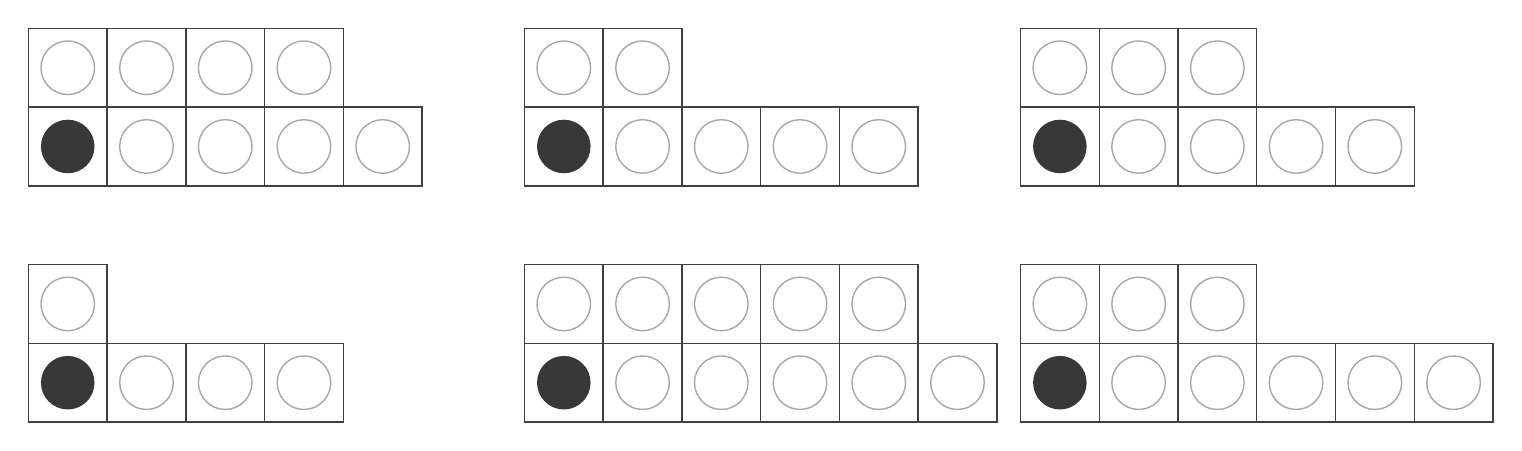
\begin{tikzpicture}[x=1mm, y=1mm]
\draw[line width=0.5pt, black!75] (0,-20) rectangle ++(10,10);
\fill[black!78] (5,-15) circle (3.4);
\draw[line width=0.5pt, black!75] (10,-20) rectangle ++(10,10);
\draw[line width=0.5pt, black!35] (15,-15) circle (3.4);
\draw[line width=0.5pt, black!75] (20,-20) rectangle ++(10,10);
\draw[line width=0.5pt, black!35] (25,-15) circle (3.4);
\draw[line width=0.5pt, black!75] (30,-20) rectangle ++(10,10);
\draw[line width=0.5pt, black!35] (35,-15) circle (3.4);
\draw[line width=0.5pt, black!75] (40,-20) rectangle ++(10,10);
\draw[line width=0.5pt, black!35] (45,-15) circle (3.4);
\draw[line width=0.5pt, black!75] (0,-10) rectangle ++(10,10);
\draw[line width=0.5pt, black!35] (5,-5) circle (3.4);
\draw[line width=0.5pt, black!75] (10,-10) rectangle ++(10,10);
\draw[line width=0.5pt, black!35] (15,-5) circle (3.4);
\draw[line width=0.5pt, black!75] (20,-10) rectangle ++(10,10);
\draw[line width=0.5pt, black!35] (25,-5) circle (3.4);
\draw[line width=0.5pt, black!75] (30,-10) rectangle ++(10,10);
\draw[line width=0.5pt, black!35] (35,-5) circle (3.4);
\draw[line width=0.5pt, black!75] (63,-20) rectangle ++(10,10);
\fill[black!78] (68,-15) circle (3.4);
\draw[line width=0.5pt, black!75] (73,-20) rectangle ++(10,10);
\draw[line width=0.5pt, black!35] (78,-15) circle (3.4);
\draw[line width=0.5pt, black!75] (83,-20) rectangle ++(10,10);
\draw[line width=0.5pt, black!35] (88,-15) circle (3.4);
\draw[line width=0.5pt, black!75] (93,-20) rectangle ++(10,10);
\draw[line width=0.5pt, black!35] (98,-15) circle (3.4);
\draw[line width=0.5pt, black!75] (103,-20) rectangle ++(10,10);
\draw[line width=0.5pt, black!35] (108,-15) circle (3.4);
\draw[line width=0.5pt, black!75] (63,-10) rectangle ++(10,10);
\draw[line width=0.5pt, black!35] (68,-5) circle (3.4);
\draw[line width=0.5pt, black!75] (73,-10) rectangle ++(10,10);
\draw[line width=0.5pt, black!35] (78,-5) circle (3.4);
\draw[line width=0.5pt, black!75] (126,-20) rectangle ++(10,10);
\fill[black!78] (131,-15) circle (3.4);
\draw[line width=0.5pt, black!75] (136,-20) rectangle ++(10,10);
\draw[line width=0.5pt, black!35] (141,-15) circle (3.4);
\draw[line width=0.5pt, black!75] (146,-20) rectangle ++(10,10);
\draw[line width=0.5pt, black!35] (151,-15) circle (3.4);
\draw[line width=0.5pt, black!75] (156,-20) rectangle ++(10,10);
\draw[line width=0.5pt, black!35] (161,-15) circle (3.4);
\draw[line width=0.5pt, black!75] (166,-20) rectangle ++(10,10);
\draw[line width=0.5pt, black!35] (171,-15) circle (3.4);
\draw[line width=0.5pt, black!75] (126,-10) rectangle ++(10,10);
\draw[line width=0.5pt, black!35] (131,-5) circle (3.4);
\draw[line width=0.5pt, black!75] (136,-10) rectangle ++(10,10);
\draw[line width=0.5pt, black!35] (141,-5) circle (3.4);
\draw[line width=0.5pt, black!75] (146,-10) rectangle ++(10,10);
\draw[line width=0.5pt, black!35] (151,-5) circle (3.4);
\draw[line width=0.5pt, black!75] (0,-50) rectangle ++(10,10);
\fill[black!78] (5,-45) circle (3.4);
\draw[line width=0.5pt, black!75] (10,-50) rectangle ++(10,10);
\draw[line width=0.5pt, black!35] (15,-45) circle (3.4);
\draw[line width=0.5pt, black!75] (20,-50) rectangle ++(10,10);
\draw[line width=0.5pt, black!35] (25,-45) circle (3.4);
\draw[line width=0.5pt, black!75] (30,-50) rectangle ++(10,10);
\draw[line width=0.5pt, black!35] (35,-45) circle (3.4);
\draw[line width=0.5pt, black!75] (0,-40) rectangle ++(10,10);
\draw[line width=0.5pt, black!35] (5,-35) circle (3.4);
\draw[line width=0.5pt, black!75] (63,-50) rectangle ++(10,10);
\fill[black!78] (68,-45) circle (3.4);
\draw[line width=0.5pt, black!75] (73,-50) rectangle ++(10,10);
\draw[line width=0.5pt, black!35] (78,-45) circle (3.4);
\draw[line width=0.5pt, black!75] (83,-50) rectangle ++(10,10);
\draw[line width=0.5pt, black!35] (88,-45) circle (3.4);
\draw[line width=0.5pt, black!75] (93,-50) rectangle ++(10,10);
\draw[line width=0.5pt, black!35] (98,-45) circle (3.4);
\draw[line width=0.5pt, black!75] (103,-50) rectangle ++(10,10);
\draw[line width=0.5pt, black!35] (108,-45) circle (3.4);
\draw[line width=0.5pt, black!75] (113,-50) rectangle ++(10,10);
\draw[line width=0.5pt, black!35] (118,-45) circle (3.4);
\draw[line width=0.5pt, black!75] (63,-40) rectangle ++(10,10);
\draw[line width=0.5pt, black!35] (68,-35) circle (3.4);
\draw[line width=0.5pt, black!75] (73,-40) rectangle ++(10,10);
\draw[line width=0.5pt, black!35] (78,-35) circle (3.4);
\draw[line width=0.5pt, black!75] (83,-40) rectangle ++(10,10);
\draw[line width=0.5pt, black!35] (88,-35) circle (3.4);
\draw[line width=0.5pt, black!75] (93,-40) rectangle ++(10,10);
\draw[line width=0.5pt, black!35] (98,-35) circle (3.4);
\draw[line width=0.5pt, black!75] (103,-40) rectangle ++(10,10);
\draw[line width=0.5pt, black!35] (108,-35) circle (3.4);
\draw[line width=0.5pt, black!75] (126,-50) rectangle ++(10,10);
\fill[black!78] (131,-45) circle (3.4);
\draw[line width=0.5pt, black!75] (136,-50) rectangle ++(10,10);
\draw[line width=0.5pt, black!35] (141,-45) circle (3.4);
\draw[line width=0.5pt, black!75] (146,-50) rectangle ++(10,10);
\draw[line width=0.5pt, black!35] (151,-45) circle (3.4);
\draw[line width=0.5pt, black!75] (156,-50) rectangle ++(10,10);
\draw[line width=0.5pt, black!35] (161,-45) circle (3.4);
\draw[line width=0.5pt, black!75] (166,-50) rectangle ++(10,10);
\draw[line width=0.5pt, black!35] (171,-45) circle (3.4);
\draw[line width=0.5pt, black!75] (176,-50) rectangle ++(10,10);
\draw[line width=0.5pt, black!35] (181,-45) circle (3.4);
\draw[line width=0.5pt, black!75] (126,-40) rectangle ++(10,10);
\draw[line width=0.5pt, black!35] (131,-35) circle (3.4);
\draw[line width=0.5pt, black!75] (136,-40) rectangle ++(10,10);
\draw[line width=0.5pt, black!35] (141,-35) circle (3.4);
\draw[line width=0.5pt, black!75] (146,-40) rectangle ++(10,10);
\draw[line width=0.5pt, black!35] (151,-35) circle (3.4);
\end{tikzpicture}\par\vspace{0mm}
\newpage
\prob{4}On each board, mark a first bite after which the first player can make sure to win.\par\vspace{5mm}
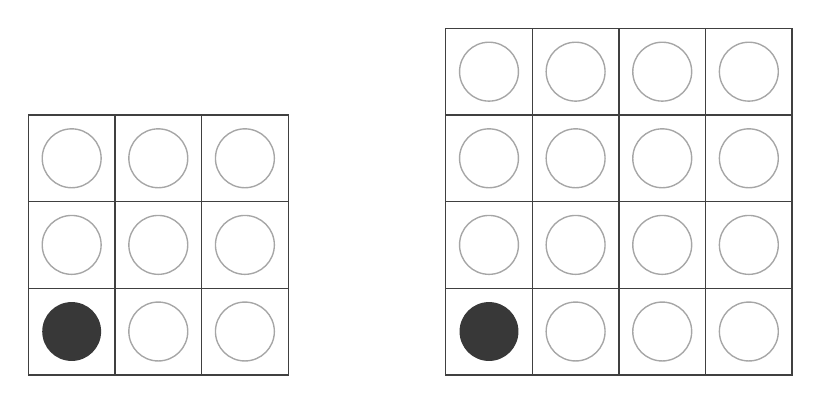
\begin{tikzpicture}[x=1mm, y=1mm]
\draw[line width=0.5pt, black!75] (0,0) rectangle ++(11,11);
\fill[black!78] (5.5,5.5) circle (3.74);
\draw[line width=0.5pt, black!75] (11,0) rectangle ++(11,11);
\draw[line width=0.5pt, black!35] (16.5,5.5) circle (3.74);
\draw[line width=0.5pt, black!75] (22,0) rectangle ++(11,11);
\draw[line width=0.5pt, black!35] (27.5,5.5) circle (3.74);
\draw[line width=0.5pt, black!75] (0,11) rectangle ++(11,11);
\draw[line width=0.5pt, black!35] (5.5,16.5) circle (3.74);
\draw[line width=0.5pt, black!75] (11,11) rectangle ++(11,11);
\draw[line width=0.5pt, black!35] (16.5,16.5) circle (3.74);
\draw[line width=0.5pt, black!75] (22,11) rectangle ++(11,11);
\draw[line width=0.5pt, black!35] (27.5,16.5) circle (3.74);
\draw[line width=0.5pt, black!75] (0,22) rectangle ++(11,11);
\draw[line width=0.5pt, black!35] (5.5,27.5) circle (3.74);
\draw[line width=0.5pt, black!75] (11,22) rectangle ++(11,11);
\draw[line width=0.5pt, black!35] (16.5,27.5) circle (3.74);
\draw[line width=0.5pt, black!75] (22,22) rectangle ++(11,11);
\draw[line width=0.5pt, black!35] (27.5,27.5) circle (3.74);
\draw[line width=0.5pt, black!75] (53,0) rectangle ++(11,11);
\fill[black!78] (58.5,5.5) circle (3.74);
\draw[line width=0.5pt, black!75] (64,0) rectangle ++(11,11);
\draw[line width=0.5pt, black!35] (69.5,5.5) circle (3.74);
\draw[line width=0.5pt, black!75] (75,0) rectangle ++(11,11);
\draw[line width=0.5pt, black!35] (80.5,5.5) circle (3.74);
\draw[line width=0.5pt, black!75] (86,0) rectangle ++(11,11);
\draw[line width=0.5pt, black!35] (91.5,5.5) circle (3.74);
\draw[line width=0.5pt, black!75] (53,11) rectangle ++(11,11);
\draw[line width=0.5pt, black!35] (58.5,16.5) circle (3.74);
\draw[line width=0.5pt, black!75] (64,11) rectangle ++(11,11);
\draw[line width=0.5pt, black!35] (69.5,16.5) circle (3.74);
\draw[line width=0.5pt, black!75] (75,11) rectangle ++(11,11);
\draw[line width=0.5pt, black!35] (80.5,16.5) circle (3.74);
\draw[line width=0.5pt, black!75] (86,11) rectangle ++(11,11);
\draw[line width=0.5pt, black!35] (91.5,16.5) circle (3.74);
\draw[line width=0.5pt, black!75] (53,22) rectangle ++(11,11);
\draw[line width=0.5pt, black!35] (58.5,27.5) circle (3.74);
\draw[line width=0.5pt, black!75] (64,22) rectangle ++(11,11);
\draw[line width=0.5pt, black!35] (69.5,27.5) circle (3.74);
\draw[line width=0.5pt, black!75] (75,22) rectangle ++(11,11);
\draw[line width=0.5pt, black!35] (80.5,27.5) circle (3.74);
\draw[line width=0.5pt, black!75] (86,22) rectangle ++(11,11);
\draw[line width=0.5pt, black!35] (91.5,27.5) circle (3.74);
\draw[line width=0.5pt, black!75] (53,33) rectangle ++(11,11);
\draw[line width=0.5pt, black!35] (58.5,38.5) circle (3.74);
\draw[line width=0.5pt, black!75] (64,33) rectangle ++(11,11);
\draw[line width=0.5pt, black!35] (69.5,38.5) circle (3.74);
\draw[line width=0.5pt, black!75] (75,33) rectangle ++(11,11);
\draw[line width=0.5pt, black!35] (80.5,38.5) circle (3.74);
\draw[line width=0.5pt, black!75] (86,33) rectangle ++(11,11);
\draw[line width=0.5pt, black!35] (91.5,38.5) circle (3.74);
\end{tikzpicture}\par\vspace{18mm}
\prob{5}Explain how the first player can make sure to win on every square board bigger than one cookie, even this 10 by 10 one.\par\vspace{5mm}
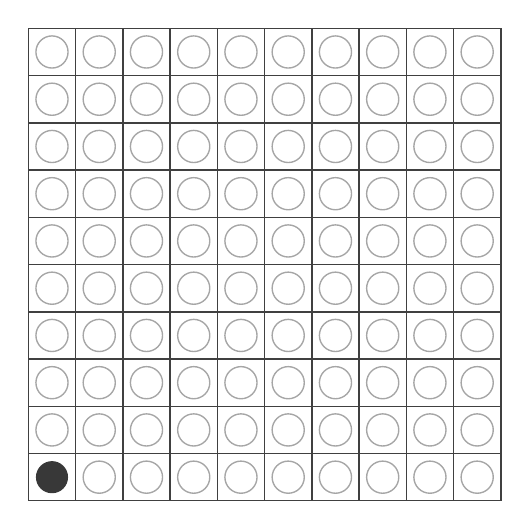
\begin{tikzpicture}[x=1mm, y=1mm]
\draw[line width=0.5pt, black!75] (0,0) rectangle ++(6,6);
\fill[black!78] (3,3) circle (2.04);
\draw[line width=0.5pt, black!75] (6,0) rectangle ++(6,6);
\draw[line width=0.5pt, black!35] (9,3) circle (2.04);
\draw[line width=0.5pt, black!75] (12,0) rectangle ++(6,6);
\draw[line width=0.5pt, black!35] (15,3) circle (2.04);
\draw[line width=0.5pt, black!75] (18,0) rectangle ++(6,6);
\draw[line width=0.5pt, black!35] (21,3) circle (2.04);
\draw[line width=0.5pt, black!75] (24,0) rectangle ++(6,6);
\draw[line width=0.5pt, black!35] (27,3) circle (2.04);
\draw[line width=0.5pt, black!75] (30,0) rectangle ++(6,6);
\draw[line width=0.5pt, black!35] (33,3) circle (2.04);
\draw[line width=0.5pt, black!75] (36,0) rectangle ++(6,6);
\draw[line width=0.5pt, black!35] (39,3) circle (2.04);
\draw[line width=0.5pt, black!75] (42,0) rectangle ++(6,6);
\draw[line width=0.5pt, black!35] (45,3) circle (2.04);
\draw[line width=0.5pt, black!75] (48,0) rectangle ++(6,6);
\draw[line width=0.5pt, black!35] (51,3) circle (2.04);
\draw[line width=0.5pt, black!75] (54,0) rectangle ++(6,6);
\draw[line width=0.5pt, black!35] (57,3) circle (2.04);
\draw[line width=0.5pt, black!75] (0,6) rectangle ++(6,6);
\draw[line width=0.5pt, black!35] (3,9) circle (2.04);
\draw[line width=0.5pt, black!75] (6,6) rectangle ++(6,6);
\draw[line width=0.5pt, black!35] (9,9) circle (2.04);
\draw[line width=0.5pt, black!75] (12,6) rectangle ++(6,6);
\draw[line width=0.5pt, black!35] (15,9) circle (2.04);
\draw[line width=0.5pt, black!75] (18,6) rectangle ++(6,6);
\draw[line width=0.5pt, black!35] (21,9) circle (2.04);
\draw[line width=0.5pt, black!75] (24,6) rectangle ++(6,6);
\draw[line width=0.5pt, black!35] (27,9) circle (2.04);
\draw[line width=0.5pt, black!75] (30,6) rectangle ++(6,6);
\draw[line width=0.5pt, black!35] (33,9) circle (2.04);
\draw[line width=0.5pt, black!75] (36,6) rectangle ++(6,6);
\draw[line width=0.5pt, black!35] (39,9) circle (2.04);
\draw[line width=0.5pt, black!75] (42,6) rectangle ++(6,6);
\draw[line width=0.5pt, black!35] (45,9) circle (2.04);
\draw[line width=0.5pt, black!75] (48,6) rectangle ++(6,6);
\draw[line width=0.5pt, black!35] (51,9) circle (2.04);
\draw[line width=0.5pt, black!75] (54,6) rectangle ++(6,6);
\draw[line width=0.5pt, black!35] (57,9) circle (2.04);
\draw[line width=0.5pt, black!75] (0,12) rectangle ++(6,6);
\draw[line width=0.5pt, black!35] (3,15) circle (2.04);
\draw[line width=0.5pt, black!75] (6,12) rectangle ++(6,6);
\draw[line width=0.5pt, black!35] (9,15) circle (2.04);
\draw[line width=0.5pt, black!75] (12,12) rectangle ++(6,6);
\draw[line width=0.5pt, black!35] (15,15) circle (2.04);
\draw[line width=0.5pt, black!75] (18,12) rectangle ++(6,6);
\draw[line width=0.5pt, black!35] (21,15) circle (2.04);
\draw[line width=0.5pt, black!75] (24,12) rectangle ++(6,6);
\draw[line width=0.5pt, black!35] (27,15) circle (2.04);
\draw[line width=0.5pt, black!75] (30,12) rectangle ++(6,6);
\draw[line width=0.5pt, black!35] (33,15) circle (2.04);
\draw[line width=0.5pt, black!75] (36,12) rectangle ++(6,6);
\draw[line width=0.5pt, black!35] (39,15) circle (2.04);
\draw[line width=0.5pt, black!75] (42,12) rectangle ++(6,6);
\draw[line width=0.5pt, black!35] (45,15) circle (2.04);
\draw[line width=0.5pt, black!75] (48,12) rectangle ++(6,6);
\draw[line width=0.5pt, black!35] (51,15) circle (2.04);
\draw[line width=0.5pt, black!75] (54,12) rectangle ++(6,6);
\draw[line width=0.5pt, black!35] (57,15) circle (2.04);
\draw[line width=0.5pt, black!75] (0,18) rectangle ++(6,6);
\draw[line width=0.5pt, black!35] (3,21) circle (2.04);
\draw[line width=0.5pt, black!75] (6,18) rectangle ++(6,6);
\draw[line width=0.5pt, black!35] (9,21) circle (2.04);
\draw[line width=0.5pt, black!75] (12,18) rectangle ++(6,6);
\draw[line width=0.5pt, black!35] (15,21) circle (2.04);
\draw[line width=0.5pt, black!75] (18,18) rectangle ++(6,6);
\draw[line width=0.5pt, black!35] (21,21) circle (2.04);
\draw[line width=0.5pt, black!75] (24,18) rectangle ++(6,6);
\draw[line width=0.5pt, black!35] (27,21) circle (2.04);
\draw[line width=0.5pt, black!75] (30,18) rectangle ++(6,6);
\draw[line width=0.5pt, black!35] (33,21) circle (2.04);
\draw[line width=0.5pt, black!75] (36,18) rectangle ++(6,6);
\draw[line width=0.5pt, black!35] (39,21) circle (2.04);
\draw[line width=0.5pt, black!75] (42,18) rectangle ++(6,6);
\draw[line width=0.5pt, black!35] (45,21) circle (2.04);
\draw[line width=0.5pt, black!75] (48,18) rectangle ++(6,6);
\draw[line width=0.5pt, black!35] (51,21) circle (2.04);
\draw[line width=0.5pt, black!75] (54,18) rectangle ++(6,6);
\draw[line width=0.5pt, black!35] (57,21) circle (2.04);
\draw[line width=0.5pt, black!75] (0,24) rectangle ++(6,6);
\draw[line width=0.5pt, black!35] (3,27) circle (2.04);
\draw[line width=0.5pt, black!75] (6,24) rectangle ++(6,6);
\draw[line width=0.5pt, black!35] (9,27) circle (2.04);
\draw[line width=0.5pt, black!75] (12,24) rectangle ++(6,6);
\draw[line width=0.5pt, black!35] (15,27) circle (2.04);
\draw[line width=0.5pt, black!75] (18,24) rectangle ++(6,6);
\draw[line width=0.5pt, black!35] (21,27) circle (2.04);
\draw[line width=0.5pt, black!75] (24,24) rectangle ++(6,6);
\draw[line width=0.5pt, black!35] (27,27) circle (2.04);
\draw[line width=0.5pt, black!75] (30,24) rectangle ++(6,6);
\draw[line width=0.5pt, black!35] (33,27) circle (2.04);
\draw[line width=0.5pt, black!75] (36,24) rectangle ++(6,6);
\draw[line width=0.5pt, black!35] (39,27) circle (2.04);
\draw[line width=0.5pt, black!75] (42,24) rectangle ++(6,6);
\draw[line width=0.5pt, black!35] (45,27) circle (2.04);
\draw[line width=0.5pt, black!75] (48,24) rectangle ++(6,6);
\draw[line width=0.5pt, black!35] (51,27) circle (2.04);
\draw[line width=0.5pt, black!75] (54,24) rectangle ++(6,6);
\draw[line width=0.5pt, black!35] (57,27) circle (2.04);
\draw[line width=0.5pt, black!75] (0,30) rectangle ++(6,6);
\draw[line width=0.5pt, black!35] (3,33) circle (2.04);
\draw[line width=0.5pt, black!75] (6,30) rectangle ++(6,6);
\draw[line width=0.5pt, black!35] (9,33) circle (2.04);
\draw[line width=0.5pt, black!75] (12,30) rectangle ++(6,6);
\draw[line width=0.5pt, black!35] (15,33) circle (2.04);
\draw[line width=0.5pt, black!75] (18,30) rectangle ++(6,6);
\draw[line width=0.5pt, black!35] (21,33) circle (2.04);
\draw[line width=0.5pt, black!75] (24,30) rectangle ++(6,6);
\draw[line width=0.5pt, black!35] (27,33) circle (2.04);
\draw[line width=0.5pt, black!75] (30,30) rectangle ++(6,6);
\draw[line width=0.5pt, black!35] (33,33) circle (2.04);
\draw[line width=0.5pt, black!75] (36,30) rectangle ++(6,6);
\draw[line width=0.5pt, black!35] (39,33) circle (2.04);
\draw[line width=0.5pt, black!75] (42,30) rectangle ++(6,6);
\draw[line width=0.5pt, black!35] (45,33) circle (2.04);
\draw[line width=0.5pt, black!75] (48,30) rectangle ++(6,6);
\draw[line width=0.5pt, black!35] (51,33) circle (2.04);
\draw[line width=0.5pt, black!75] (54,30) rectangle ++(6,6);
\draw[line width=0.5pt, black!35] (57,33) circle (2.04);
\draw[line width=0.5pt, black!75] (0,36) rectangle ++(6,6);
\draw[line width=0.5pt, black!35] (3,39) circle (2.04);
\draw[line width=0.5pt, black!75] (6,36) rectangle ++(6,6);
\draw[line width=0.5pt, black!35] (9,39) circle (2.04);
\draw[line width=0.5pt, black!75] (12,36) rectangle ++(6,6);
\draw[line width=0.5pt, black!35] (15,39) circle (2.04);
\draw[line width=0.5pt, black!75] (18,36) rectangle ++(6,6);
\draw[line width=0.5pt, black!35] (21,39) circle (2.04);
\draw[line width=0.5pt, black!75] (24,36) rectangle ++(6,6);
\draw[line width=0.5pt, black!35] (27,39) circle (2.04);
\draw[line width=0.5pt, black!75] (30,36) rectangle ++(6,6);
\draw[line width=0.5pt, black!35] (33,39) circle (2.04);
\draw[line width=0.5pt, black!75] (36,36) rectangle ++(6,6);
\draw[line width=0.5pt, black!35] (39,39) circle (2.04);
\draw[line width=0.5pt, black!75] (42,36) rectangle ++(6,6);
\draw[line width=0.5pt, black!35] (45,39) circle (2.04);
\draw[line width=0.5pt, black!75] (48,36) rectangle ++(6,6);
\draw[line width=0.5pt, black!35] (51,39) circle (2.04);
\draw[line width=0.5pt, black!75] (54,36) rectangle ++(6,6);
\draw[line width=0.5pt, black!35] (57,39) circle (2.04);
\draw[line width=0.5pt, black!75] (0,42) rectangle ++(6,6);
\draw[line width=0.5pt, black!35] (3,45) circle (2.04);
\draw[line width=0.5pt, black!75] (6,42) rectangle ++(6,6);
\draw[line width=0.5pt, black!35] (9,45) circle (2.04);
\draw[line width=0.5pt, black!75] (12,42) rectangle ++(6,6);
\draw[line width=0.5pt, black!35] (15,45) circle (2.04);
\draw[line width=0.5pt, black!75] (18,42) rectangle ++(6,6);
\draw[line width=0.5pt, black!35] (21,45) circle (2.04);
\draw[line width=0.5pt, black!75] (24,42) rectangle ++(6,6);
\draw[line width=0.5pt, black!35] (27,45) circle (2.04);
\draw[line width=0.5pt, black!75] (30,42) rectangle ++(6,6);
\draw[line width=0.5pt, black!35] (33,45) circle (2.04);
\draw[line width=0.5pt, black!75] (36,42) rectangle ++(6,6);
\draw[line width=0.5pt, black!35] (39,45) circle (2.04);
\draw[line width=0.5pt, black!75] (42,42) rectangle ++(6,6);
\draw[line width=0.5pt, black!35] (45,45) circle (2.04);
\draw[line width=0.5pt, black!75] (48,42) rectangle ++(6,6);
\draw[line width=0.5pt, black!35] (51,45) circle (2.04);
\draw[line width=0.5pt, black!75] (54,42) rectangle ++(6,6);
\draw[line width=0.5pt, black!35] (57,45) circle (2.04);
\draw[line width=0.5pt, black!75] (0,48) rectangle ++(6,6);
\draw[line width=0.5pt, black!35] (3,51) circle (2.04);
\draw[line width=0.5pt, black!75] (6,48) rectangle ++(6,6);
\draw[line width=0.5pt, black!35] (9,51) circle (2.04);
\draw[line width=0.5pt, black!75] (12,48) rectangle ++(6,6);
\draw[line width=0.5pt, black!35] (15,51) circle (2.04);
\draw[line width=0.5pt, black!75] (18,48) rectangle ++(6,6);
\draw[line width=0.5pt, black!35] (21,51) circle (2.04);
\draw[line width=0.5pt, black!75] (24,48) rectangle ++(6,6);
\draw[line width=0.5pt, black!35] (27,51) circle (2.04);
\draw[line width=0.5pt, black!75] (30,48) rectangle ++(6,6);
\draw[line width=0.5pt, black!35] (33,51) circle (2.04);
\draw[line width=0.5pt, black!75] (36,48) rectangle ++(6,6);
\draw[line width=0.5pt, black!35] (39,51) circle (2.04);
\draw[line width=0.5pt, black!75] (42,48) rectangle ++(6,6);
\draw[line width=0.5pt, black!35] (45,51) circle (2.04);
\draw[line width=0.5pt, black!75] (48,48) rectangle ++(6,6);
\draw[line width=0.5pt, black!35] (51,51) circle (2.04);
\draw[line width=0.5pt, black!75] (54,48) rectangle ++(6,6);
\draw[line width=0.5pt, black!35] (57,51) circle (2.04);
\draw[line width=0.5pt, black!75] (0,54) rectangle ++(6,6);
\draw[line width=0.5pt, black!35] (3,57) circle (2.04);
\draw[line width=0.5pt, black!75] (6,54) rectangle ++(6,6);
\draw[line width=0.5pt, black!35] (9,57) circle (2.04);
\draw[line width=0.5pt, black!75] (12,54) rectangle ++(6,6);
\draw[line width=0.5pt, black!35] (15,57) circle (2.04);
\draw[line width=0.5pt, black!75] (18,54) rectangle ++(6,6);
\draw[line width=0.5pt, black!35] (21,57) circle (2.04);
\draw[line width=0.5pt, black!75] (24,54) rectangle ++(6,6);
\draw[line width=0.5pt, black!35] (27,57) circle (2.04);
\draw[line width=0.5pt, black!75] (30,54) rectangle ++(6,6);
\draw[line width=0.5pt, black!35] (33,57) circle (2.04);
\draw[line width=0.5pt, black!75] (36,54) rectangle ++(6,6);
\draw[line width=0.5pt, black!35] (39,57) circle (2.04);
\draw[line width=0.5pt, black!75] (42,54) rectangle ++(6,6);
\draw[line width=0.5pt, black!35] (45,57) circle (2.04);
\draw[line width=0.5pt, black!75] (48,54) rectangle ++(6,6);
\draw[line width=0.5pt, black!35] (51,57) circle (2.04);
\draw[line width=0.5pt, black!75] (54,54) rectangle ++(6,6);
\draw[line width=0.5pt, black!35] (57,57) circle (2.04);
\end{tikzpicture}\par\vspace{0mm}
\newpage
\prob{6}On the 3 by 4 board, mark a first bite after which the first player can make sure to win.\par\vspace{5mm}
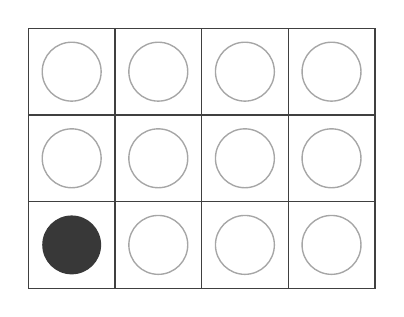
\begin{tikzpicture}[x=1mm, y=1mm]
\draw[line width=0.5pt, black!75] (0,0) rectangle ++(11,11);
\fill[black!78] (5.5,5.5) circle (3.74);
\draw[line width=0.5pt, black!75] (11,0) rectangle ++(11,11);
\draw[line width=0.5pt, black!35] (16.5,5.5) circle (3.74);
\draw[line width=0.5pt, black!75] (22,0) rectangle ++(11,11);
\draw[line width=0.5pt, black!35] (27.5,5.5) circle (3.74);
\draw[line width=0.5pt, black!75] (33,0) rectangle ++(11,11);
\draw[line width=0.5pt, black!35] (38.5,5.5) circle (3.74);
\draw[line width=0.5pt, black!75] (0,11) rectangle ++(11,11);
\draw[line width=0.5pt, black!35] (5.5,16.5) circle (3.74);
\draw[line width=0.5pt, black!75] (11,11) rectangle ++(11,11);
\draw[line width=0.5pt, black!35] (16.5,16.5) circle (3.74);
\draw[line width=0.5pt, black!75] (22,11) rectangle ++(11,11);
\draw[line width=0.5pt, black!35] (27.5,16.5) circle (3.74);
\draw[line width=0.5pt, black!75] (33,11) rectangle ++(11,11);
\draw[line width=0.5pt, black!35] (38.5,16.5) circle (3.74);
\draw[line width=0.5pt, black!75] (0,22) rectangle ++(11,11);
\draw[line width=0.5pt, black!35] (5.5,27.5) circle (3.74);
\draw[line width=0.5pt, black!75] (11,22) rectangle ++(11,11);
\draw[line width=0.5pt, black!35] (16.5,27.5) circle (3.74);
\draw[line width=0.5pt, black!75] (22,22) rectangle ++(11,11);
\draw[line width=0.5pt, black!35] (27.5,27.5) circle (3.74);
\draw[line width=0.5pt, black!75] (33,22) rectangle ++(11,11);
\draw[line width=0.5pt, black!35] (38.5,27.5) circle (3.74);
\end{tikzpicture}\par\vspace{0mm}
\newpage
\prob{7}Take bites from a full 3 by 5 board to make boards with three rows where the player who goes second can make sure to win. Color each one you find on a grid.\par\vspace{8mm}
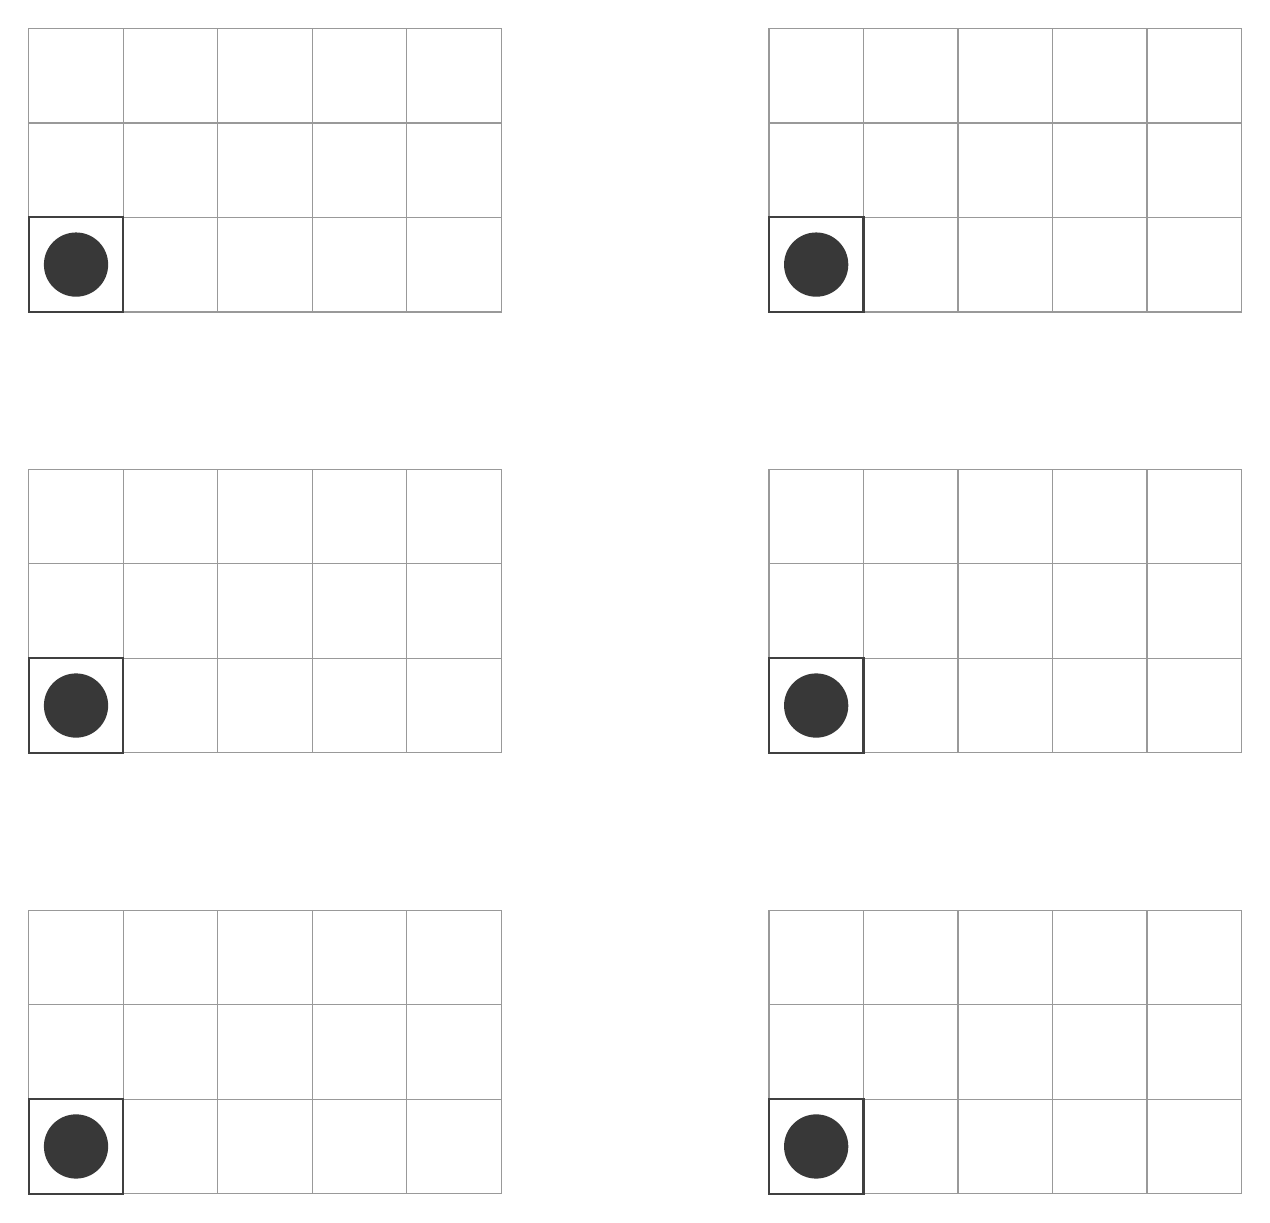
\begin{tikzpicture}[x=1mm, y=1mm]
\draw[line width=0.5pt, black!40] (0,0) rectangle ++(12,12);
\draw[line width=0.5pt, black!40] (12,0) rectangle ++(12,12);
\draw[line width=0.5pt, black!40] (24,0) rectangle ++(12,12);
\draw[line width=0.5pt, black!40] (36,0) rectangle ++(12,12);
\draw[line width=0.5pt, black!40] (48,0) rectangle ++(12,12);
\draw[line width=0.5pt, black!40] (0,12) rectangle ++(12,12);
\draw[line width=0.5pt, black!40] (12,12) rectangle ++(12,12);
\draw[line width=0.5pt, black!40] (24,12) rectangle ++(12,12);
\draw[line width=0.5pt, black!40] (36,12) rectangle ++(12,12);
\draw[line width=0.5pt, black!40] (48,12) rectangle ++(12,12);
\draw[line width=0.5pt, black!40] (0,24) rectangle ++(12,12);
\draw[line width=0.5pt, black!40] (12,24) rectangle ++(12,12);
\draw[line width=0.5pt, black!40] (24,24) rectangle ++(12,12);
\draw[line width=0.5pt, black!40] (36,24) rectangle ++(12,12);
\draw[line width=0.5pt, black!40] (48,24) rectangle ++(12,12);
\fill[black!78] (6,6) circle (4.08);
\draw[line width=0.8pt, black!75] (0,0) rectangle ++(12,12);
\draw[line width=0.5pt, black!40] (94,0) rectangle ++(12,12);
\draw[line width=0.5pt, black!40] (106,0) rectangle ++(12,12);
\draw[line width=0.5pt, black!40] (118,0) rectangle ++(12,12);
\draw[line width=0.5pt, black!40] (130,0) rectangle ++(12,12);
\draw[line width=0.5pt, black!40] (142,0) rectangle ++(12,12);
\draw[line width=0.5pt, black!40] (94,12) rectangle ++(12,12);
\draw[line width=0.5pt, black!40] (106,12) rectangle ++(12,12);
\draw[line width=0.5pt, black!40] (118,12) rectangle ++(12,12);
\draw[line width=0.5pt, black!40] (130,12) rectangle ++(12,12);
\draw[line width=0.5pt, black!40] (142,12) rectangle ++(12,12);
\draw[line width=0.5pt, black!40] (94,24) rectangle ++(12,12);
\draw[line width=0.5pt, black!40] (106,24) rectangle ++(12,12);
\draw[line width=0.5pt, black!40] (118,24) rectangle ++(12,12);
\draw[line width=0.5pt, black!40] (130,24) rectangle ++(12,12);
\draw[line width=0.5pt, black!40] (142,24) rectangle ++(12,12);
\fill[black!78] (100,6) circle (4.08);
\draw[line width=0.8pt, black!75] (94,0) rectangle ++(12,12);
\draw[line width=0.5pt, black!40] (0,-56) rectangle ++(12,12);
\draw[line width=0.5pt, black!40] (12,-56) rectangle ++(12,12);
\draw[line width=0.5pt, black!40] (24,-56) rectangle ++(12,12);
\draw[line width=0.5pt, black!40] (36,-56) rectangle ++(12,12);
\draw[line width=0.5pt, black!40] (48,-56) rectangle ++(12,12);
\draw[line width=0.5pt, black!40] (0,-44) rectangle ++(12,12);
\draw[line width=0.5pt, black!40] (12,-44) rectangle ++(12,12);
\draw[line width=0.5pt, black!40] (24,-44) rectangle ++(12,12);
\draw[line width=0.5pt, black!40] (36,-44) rectangle ++(12,12);
\draw[line width=0.5pt, black!40] (48,-44) rectangle ++(12,12);
\draw[line width=0.5pt, black!40] (0,-32) rectangle ++(12,12);
\draw[line width=0.5pt, black!40] (12,-32) rectangle ++(12,12);
\draw[line width=0.5pt, black!40] (24,-32) rectangle ++(12,12);
\draw[line width=0.5pt, black!40] (36,-32) rectangle ++(12,12);
\draw[line width=0.5pt, black!40] (48,-32) rectangle ++(12,12);
\fill[black!78] (6,-50) circle (4.08);
\draw[line width=0.8pt, black!75] (0,-56) rectangle ++(12,12);
\draw[line width=0.5pt, black!40] (94,-56) rectangle ++(12,12);
\draw[line width=0.5pt, black!40] (106,-56) rectangle ++(12,12);
\draw[line width=0.5pt, black!40] (118,-56) rectangle ++(12,12);
\draw[line width=0.5pt, black!40] (130,-56) rectangle ++(12,12);
\draw[line width=0.5pt, black!40] (142,-56) rectangle ++(12,12);
\draw[line width=0.5pt, black!40] (94,-44) rectangle ++(12,12);
\draw[line width=0.5pt, black!40] (106,-44) rectangle ++(12,12);
\draw[line width=0.5pt, black!40] (118,-44) rectangle ++(12,12);
\draw[line width=0.5pt, black!40] (130,-44) rectangle ++(12,12);
\draw[line width=0.5pt, black!40] (142,-44) rectangle ++(12,12);
\draw[line width=0.5pt, black!40] (94,-32) rectangle ++(12,12);
\draw[line width=0.5pt, black!40] (106,-32) rectangle ++(12,12);
\draw[line width=0.5pt, black!40] (118,-32) rectangle ++(12,12);
\draw[line width=0.5pt, black!40] (130,-32) rectangle ++(12,12);
\draw[line width=0.5pt, black!40] (142,-32) rectangle ++(12,12);
\fill[black!78] (100,-50) circle (4.08);
\draw[line width=0.8pt, black!75] (94,-56) rectangle ++(12,12);
\draw[line width=0.5pt, black!40] (0,-112) rectangle ++(12,12);
\draw[line width=0.5pt, black!40] (12,-112) rectangle ++(12,12);
\draw[line width=0.5pt, black!40] (24,-112) rectangle ++(12,12);
\draw[line width=0.5pt, black!40] (36,-112) rectangle ++(12,12);
\draw[line width=0.5pt, black!40] (48,-112) rectangle ++(12,12);
\draw[line width=0.5pt, black!40] (0,-100) rectangle ++(12,12);
\draw[line width=0.5pt, black!40] (12,-100) rectangle ++(12,12);
\draw[line width=0.5pt, black!40] (24,-100) rectangle ++(12,12);
\draw[line width=0.5pt, black!40] (36,-100) rectangle ++(12,12);
\draw[line width=0.5pt, black!40] (48,-100) rectangle ++(12,12);
\draw[line width=0.5pt, black!40] (0,-88) rectangle ++(12,12);
\draw[line width=0.5pt, black!40] (12,-88) rectangle ++(12,12);
\draw[line width=0.5pt, black!40] (24,-88) rectangle ++(12,12);
\draw[line width=0.5pt, black!40] (36,-88) rectangle ++(12,12);
\draw[line width=0.5pt, black!40] (48,-88) rectangle ++(12,12);
\fill[black!78] (6,-106) circle (4.08);
\draw[line width=0.8pt, black!75] (0,-112) rectangle ++(12,12);
\draw[line width=0.5pt, black!40] (94,-112) rectangle ++(12,12);
\draw[line width=0.5pt, black!40] (106,-112) rectangle ++(12,12);
\draw[line width=0.5pt, black!40] (118,-112) rectangle ++(12,12);
\draw[line width=0.5pt, black!40] (130,-112) rectangle ++(12,12);
\draw[line width=0.5pt, black!40] (142,-112) rectangle ++(12,12);
\draw[line width=0.5pt, black!40] (94,-100) rectangle ++(12,12);
\draw[line width=0.5pt, black!40] (106,-100) rectangle ++(12,12);
\draw[line width=0.5pt, black!40] (118,-100) rectangle ++(12,12);
\draw[line width=0.5pt, black!40] (130,-100) rectangle ++(12,12);
\draw[line width=0.5pt, black!40] (142,-100) rectangle ++(12,12);
\draw[line width=0.5pt, black!40] (94,-88) rectangle ++(12,12);
\draw[line width=0.5pt, black!40] (106,-88) rectangle ++(12,12);
\draw[line width=0.5pt, black!40] (118,-88) rectangle ++(12,12);
\draw[line width=0.5pt, black!40] (130,-88) rectangle ++(12,12);
\draw[line width=0.5pt, black!40] (142,-88) rectangle ++(12,12);
\fill[black!78] (100,-106) circle (4.08);
\draw[line width=0.8pt, black!75] (94,-112) rectangle ++(12,12);
\end{tikzpicture}\par\vspace{0mm}

\end{document}
